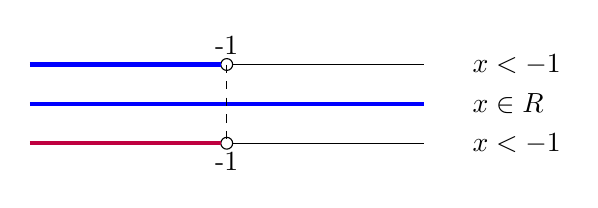
\begin{tikzpicture}[scale=0.5]
    %\draw (-11,0)-- (3,0); %AXIS
    %\foreach \x in {-1} {
    %    \draw (\x,0.5) -- (\x,-0.5) node[below] {$\x$};
    %}
    \draw (-6,1) -- (4,1);
    \draw[fill=white] (-1,1) circle (0.15) node[above]{-1};
    \node[anchor=west, right] at (5,1) {$x < -1$};
    \draw (-6,0) -- (4,0);
    \draw (-6,-1) -- (4,-1);
    \node[anchor=west, right] at (5,0) {$x \in \mathbb{R}$};
    \draw[fill=white] (-1,-1) circle (0.15) node[below]{-1};
    %\draw[thick,blue,decorate,decoration={coil,aspect=0,segment length=2.0mm}] (-7,1) -- (-1,1);
    \draw[ultra thick, blue] (-6,1) -- (-1.15,1);
    \draw[ultra thick, blue] (-6,0) -- (4,0);
    \draw[ultra thick, purple] (-6,-1) -- (-1.15,-1);
    \node[anchor=west, right] at (5,-1) {$x < -1$};
    \draw[dashed] (-1,1) -- (-1,-1);
\end{tikzpicture}
